\documentclass[11pt]{standalone}
\usepackage{tikz}
\usetikzlibrary{shapes.geometric}
\usetikzlibrary{plotmarks,shapes.multipart}
\usetikzlibrary{arrows.meta,calc,decorations.pathmorphing}
\begin{document} 

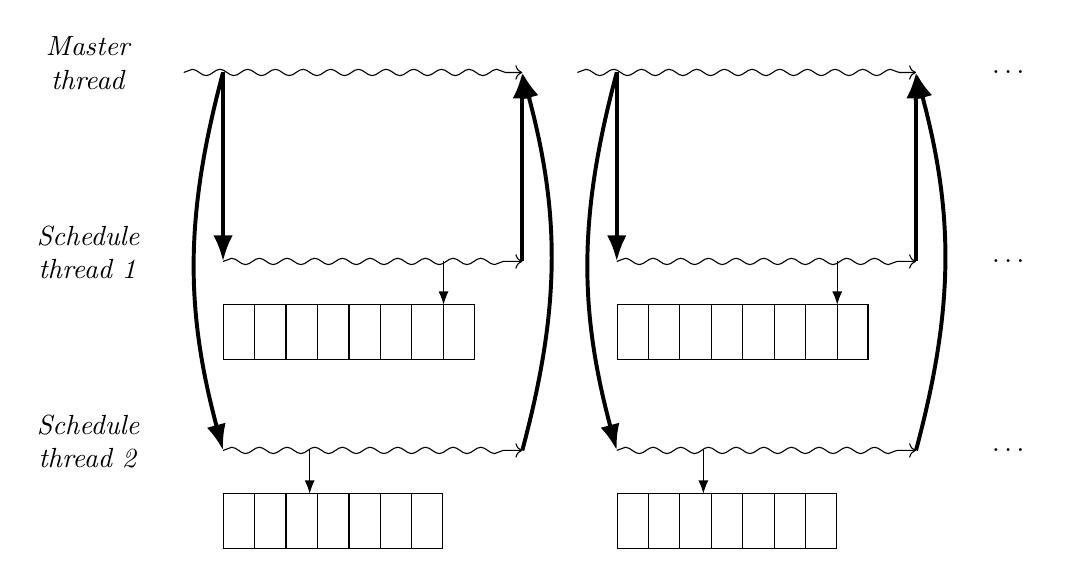
\begin{tikzpicture}


\node at(-2.7cm,-3.9cm) [label={[align=center,yshift=.7cm]south:\textit{Master}\\\textit{thread}}]{};
\draw [->,decorate,decoration={snake,pre=curveto,pre length=1,post length=1,amplitude=.4mm}] (-1.5cm,-3.9cm) -- (2.8cm,-3.9cm);


\node at(-2.7cm,-6.3cm) [label={[align=center,yshift=.7cm]south:\textit{Schedule}\\\textit{thread 1}}]{};
%\node at(0cm,-6cm) [rectangle, minimum width=6cm,minimum height=1.4cm,label={[anchor=west, yshift=-.3cm]west:{\textit{thread 1}}}] {};
\node at(-1cm,0) [rectangle split,rectangle split horizontal,rectangle split parts=8,anchor=west, draw, minimum width=5.6cm,minimum height=.7cm,yshift=-7.2cm]{};
\draw [->,decorate,decoration={snake,pre=curveto,pre length=1,post length=1,amplitude=.4mm}] (-1cm,-6.3cm) -- (2.8cm,-6.3cm);
\draw [-{Latex[]}] (1.8cm,-6.3cm) -- (1.8cm,-6.85cm);

\node at(-2.7cm,-8.7cm) [label={[align=center,yshift=.7cm]south:\textit{Schedule}\\\textit{thread 2}}]{};
%\node at(0cm,-8.4cm) [rectangle, minimum width=6cm,minimum height=1.4cm,label={[anchor=west, yshift=-.3cm]west:{\textit{thread 2}}}]{};
\node at(-1cm,0) [rectangle split,rectangle split horizontal,rectangle split parts=7,anchor=west, draw, minimum width=5.6cm,minimum height=.7cm,yshift=-9.6cm]{};
\draw [->,decorate,decoration={snake,pre=curveto,pre length=1,post length=1,amplitude=.4mm}] (-1cm,-8.7cm) -- (2.8cm,-8.7cm);
\draw [-{Latex[]}] (.1cm,-8.7cm) -- (.1cm,-9.25cm);

\path (-1cm,-3.9cm) edge[-{Latex[]},line width=.05cm] (-1cm,-6.3cm);
\path (-1cm,-3.9cm) edge[-{Latex[]},line width=.05cm, bend right=15] (-1cm,-8.7cm);

\path (2.8cm,-6.3cm) edge[-{Latex[]},line width=.05cm] (2.8cm,-3.9cm);
\path (2.8cm,-8.7cm) edge[-{Latex[]},line width=.05cm, bend right=15] (2.8cm,-3.9cm);

%\node [fill=white] at (-1.5cm,-4.8cm) {Startup};


\draw [->,decorate,decoration={snake,pre=curveto,pre length=1,post length=1,amplitude=.4mm}] (3.5cm,-3.9cm) -- (7.8cm,-3.9cm);
%\node at(0cm,-6cm) [rectangle, minimum width=6cm,minimum height=1.4cm,label={[anchor=west, yshift=-.3cm]west:{\textit{thread 1}}}] {};
\node at(4cm,0) [rectangle split,rectangle split horizontal,rectangle split parts=8,anchor=west, draw, minimum width=5.6cm,minimum height=.7cm,yshift=-7.2cm]{};
\draw [->,decorate,decoration={snake,pre=curveto,pre length=1,post length=1,amplitude=.4mm}] (4cm,-6.3cm) -- (7.8cm,-6.3cm);
\draw [-{Latex[]}] (6.8cm,-6.3cm) -- (6.8cm,-6.85cm);


%\node at(0cm,-8.4cm) [rectangle, minimum width=6cm,minimum height=1.4cm,label={[anchor=west, yshift=-.3cm]west:{\textit{thread 2}}}]{};
\node at(4cm,0) [rectangle split,rectangle split horizontal,rectangle split parts=7,anchor=west, draw, minimum width=5.6cm,minimum height=.7cm,yshift=-9.6cm]{};
\draw [->,decorate,decoration={snake,pre=curveto,pre length=1,post length=1,amplitude=.4mm}] (4cm,-8.7cm) -- (7.8cm,-8.7cm);
\draw [-{Latex[]}] (5.1cm,-8.7cm) -- (5.1cm,-9.25cm);

\path (4cm,-3.9cm) edge[-{Latex[]},line width=.05cm] (4cm,-6.3cm);
\path (4cm,-3.9cm) edge[-{Latex[]},line width=.05cm, bend right=15] (4cm,-8.7cm);

\path (7.8cm,-6.3cm) edge[-{Latex[]},line width=.05cm] (7.8cm,-3.9cm);
\path (7.8cm,-8.7cm) edge[-{Latex[]},line width=.05cm, bend right=15] (7.8cm,-3.9cm);

%\node [fill=white] at (-1.5cm,-4.8cm) {Startup};

\node at (9cm,-3.9cm) {\ldots};
\node at (9cm,-6.3cm) {\ldots};
\node at (9cm,-8.7cm) {\ldots};

\end{tikzpicture}
\end{document}